\documentclass[11pt]{extarticle}

\usepackage[english,french]{babel}
\usepackage[utf8]{inputenc}
\usepackage{url}
\usepackage[T1]{fontenc}
\usepackage{booktabs}
\usepackage{enumitem}
\usepackage{graphicx}
\usepackage{pifont}
\usepackage{makecell}
\setcellgapes{1pt}
\usepackage{placeins}
\usepackage{subcaption}
\usepackage{pgfplots}
\usetikzlibrary{calc}
\pgfplotsset{compat=1.18}
\usepgfplotslibrary{dateplot}
\usepackage[margin=1in]{geometry}
\usepackage[colorlinks=true, allcolors=blue]{hyperref}
\usepackage{amsmath}
\usepackage{pgfplotstable}
\usepackage{amsfonts}
\usepgfplotslibrary{groupplots}

\usetikzlibrary{backgrounds}

% Configuration de pgfplotstable
\pgfplotstableset{
    col sep=comma, % Colonnes séparées par des virgules
    string type,
    every head row/.style={
        before row=\toprule,
        after row=\midrule},
    every last row/.style={after row=\bottomrule},
}

\title{
    \hspace*{-12cm}
    \vspace*{1cm}
    \protect\\
    \vspace*{1cm}
    \textbf{Beyond Random Walks: Revealing the Fractal Memory of Financial Markets}
}

\author{Remiat Alexandre}

\date{\today}

\graphicspath{{img/}}

\xdefinecolor{kblue}{RGB}{0,38,69}
\xdefinecolor{korange}{RGB}{255,128,89}
\xdefinecolor{kgray}{RGB}{47,108,130}
\xdefinecolor{kgreen}{RGB}{102,143,72}


\begin{document}

\selectlanguage{english}

\maketitle


\newpage


\section*{Abstract}

This paper presents a study on long-term memory processes in financial time series using Hurst estimation methods,
specifically the traditional R/S statistic (Rescaled Range analysis) and the modified R/S statistic (M-R/S).
The R/S statistic and the modified R/S statistic are computed to determine the presence of long-term memory in the time series data.
The inferential outcomes remain inconclusive, as the computation of a solitary static Hurst exponent
across the entire time series lacks sufficient robustness and can be influenced by the length of the series, the presence of trends, or structural breaks.
To address these issues, we employed the Multifractal Detrended Fluctuation Analysis (MF-DFA) to investigate the
local behavior of the series and characterize its multifractal spectrum. The multifractal spectrum reveals that the series
might exhibit multifractal properties. To take advantage of this, we propose a trading strategy based on the Hurst
exponent, the multifractal spectrum and a proposed inefficiency index that combines the multifractality and the Hurst exponent.
We look into pairs with different patterns or behaviors that changes
when you view data at different sizes or over different time periods behavior (S\&P 500 and Russell 2000).
The inefficiency index is used as a filter to determine the significance of our trading signal.
The strategy (ModifOverlap120) outperforms the long-only S\&P 500 portfolio, the long-only Russell 2000 portfolio and
50/50 portfolio (our benchmark). Moreover, the strategies that used the inefficiency index as a filter
outperform the strategies that did not use it on Sharpe and max drawdown.



\newpage

\section{Introduction}

The Hurst exponent is a crucial tool for analyzing long-term memory and self-similarity in stochastic processes.
Originally introduced by Harold Hurst in the 1950s for studying river flows, this measure has since been widely
adopted in various fields such as physics, environmental science and finance. In financial markets, the Hurst
exponent serves as an indicator to determine whether a time series exhibits long-range dependence (a value greater
than 0.5) or mean-reverting behavior (a value less than 0.5), a value equals to 0.5 indicates that the series
follows a pure random walk, characteristic of standard Brownian motion.

The most common method for estimating the Hurst exponent is through Rescaled Range (R/S) analysis, introduced by Hurst
and later refined by Mandelbrot. However, the traditional R/S statistic has its limitations, particularly its
sensitivity to short-term memory effects, which can obscure the detection of long-term memory. To mitigate
these issues, Lo (1991) proposed a modified version of the R/S statistic (M-R/S) that better accounts for short-term autocorrelation.

In this study, we apply both the R/S method and the M-R/S to estimate the Hurst exponent on financial time series and we
complement our analysis with Multifractal Detrended Fluctuation Analysis (MF-DFA), which examines the local behavior of
the series and characterizes its multifractal spectrum.

The Fractional Brownian motion (fBm) is often used as a benchmark model for processes with memory, as it embodies the
scaling properties and persistence typically observed in long-memory data. While fBm provides a theoretical framework
for understanding these phenomena, our study focuses on practical estimation methods.

\section{Fractional Brownian Motion}

Fractional Brownian motion (fBm) is a generalization of standard Brownian motion that introduces dependence in increments,
making it suitable for modeling processes with memory effects. It is a continuous-time Gaussian process \( X_H(t) \)
where \( H \in [0, 1] \)  corresponds to the Hurst exponent with the following properties:

\begin{itemize}
    \item The process exhibits self-similarity, meaning that for any scaling factor \( c \), \( c \in \mathbb{R}^+ \), the rescaled process satisfies:
    \begin{equation}
        X_H(ct) \overset{d}{=} c^H X_H(t).
    \end{equation}
    where the symbol \(\stackrel{d}{=}\) denotes equality in distribution, meaning that the statistical properties of \(X_H(ct)\) and \(c^H X_H(t)\) are identical.

    \item The increments \( X_H(t) - X_H(s) \) follow a normal distribution with mean zero and variance :
    \begin{equation}
        \mathbb{E} \left[ (X_H(t) - X_H(s))^2 \right] = \sigma^2|t - s|^{2H},
    \end{equation}
    where \( H \) is the Hurst exponent.

    \item When \( H = 0.5 \), fBm reduces to classical Brownian motion.
    \item For \( H > 0.5 \), the process exhibits long-term positive autocorrelation, meaning that an increase in the past tends to be followed by further increases.
    \item For \( H < 0.5 \), the process has anti-persistent behavior, where an increase in the past is more likely to be followed by a decrease.
\end{itemize}

The covariance function of fBm is given by (see Section~\ref{sec:covariance_fbm} for demonstration):

\begin{equation}
    C_H(t, s) = \frac{\sigma^2}{2} \left( t^{2H} + s^{2H} - |t - s|^{2H} \right),
    \label{eq:fbm_covariance}
\end{equation}

which accounts for the dependence structure of the process. The Hurst exponent \( H \) plays a critical role in determining the smoothness and correlation properties of fBm:

\begin{itemize}
    \item \textbf{For small \( H \) values} (\( H < 0.5 \)), the process is highly erratic, with rapid changes and weak memory effects.
    \item \textbf{For large \( H \) values} (\( H > 0.5 \)), the trajectory becomes smoother, and the process exhibits long-range dependence.
\end{itemize}


\subsection{Simulation of Fractional Brownian Motion}

In this simulation, we aim to generate fractional Brownian motion (fBm) to better understand how the autocorrelation
decays as a function of the Hurst exponent \( H \). By simulating paths for different values of \( H \), we can observe
how the memory and persistence properties of the process vary.
To generate the fractional Brownian motion (fBm), we use a Cholesky decomposition-based approach. The covariance matrix of fBm is given by \eqref{eq:fbm_covariance}:

where \( H \) is the Hurst exponent, which determines the degree of long-term dependence in the process.

The steps of the simulation are as follows:
\begin{enumerate}
    \item Define a time grid of \( N \) points between \( 0 \) and \( T \).
    \item Compute the covariance matrix using \eqref{eq:fbm_covariance}.
    \item Apply Cholesky decomposition to obtain a lower triangular matrix \( L \).
    \item Generate a vector \( W \) of standard normal random variables.
    \item Obtain the fBm path by computing \( X = L W \).
\end{enumerate}

The params used for this simulation are N = 1000 number of points, T = 1 day, Hurst exponents \( H = 0.2, 0.35, 0.5, 0.65, 0.8 \), the number
of lag for the autocorrelation is 40.

\begin{figure}[!ht]
    \centering
    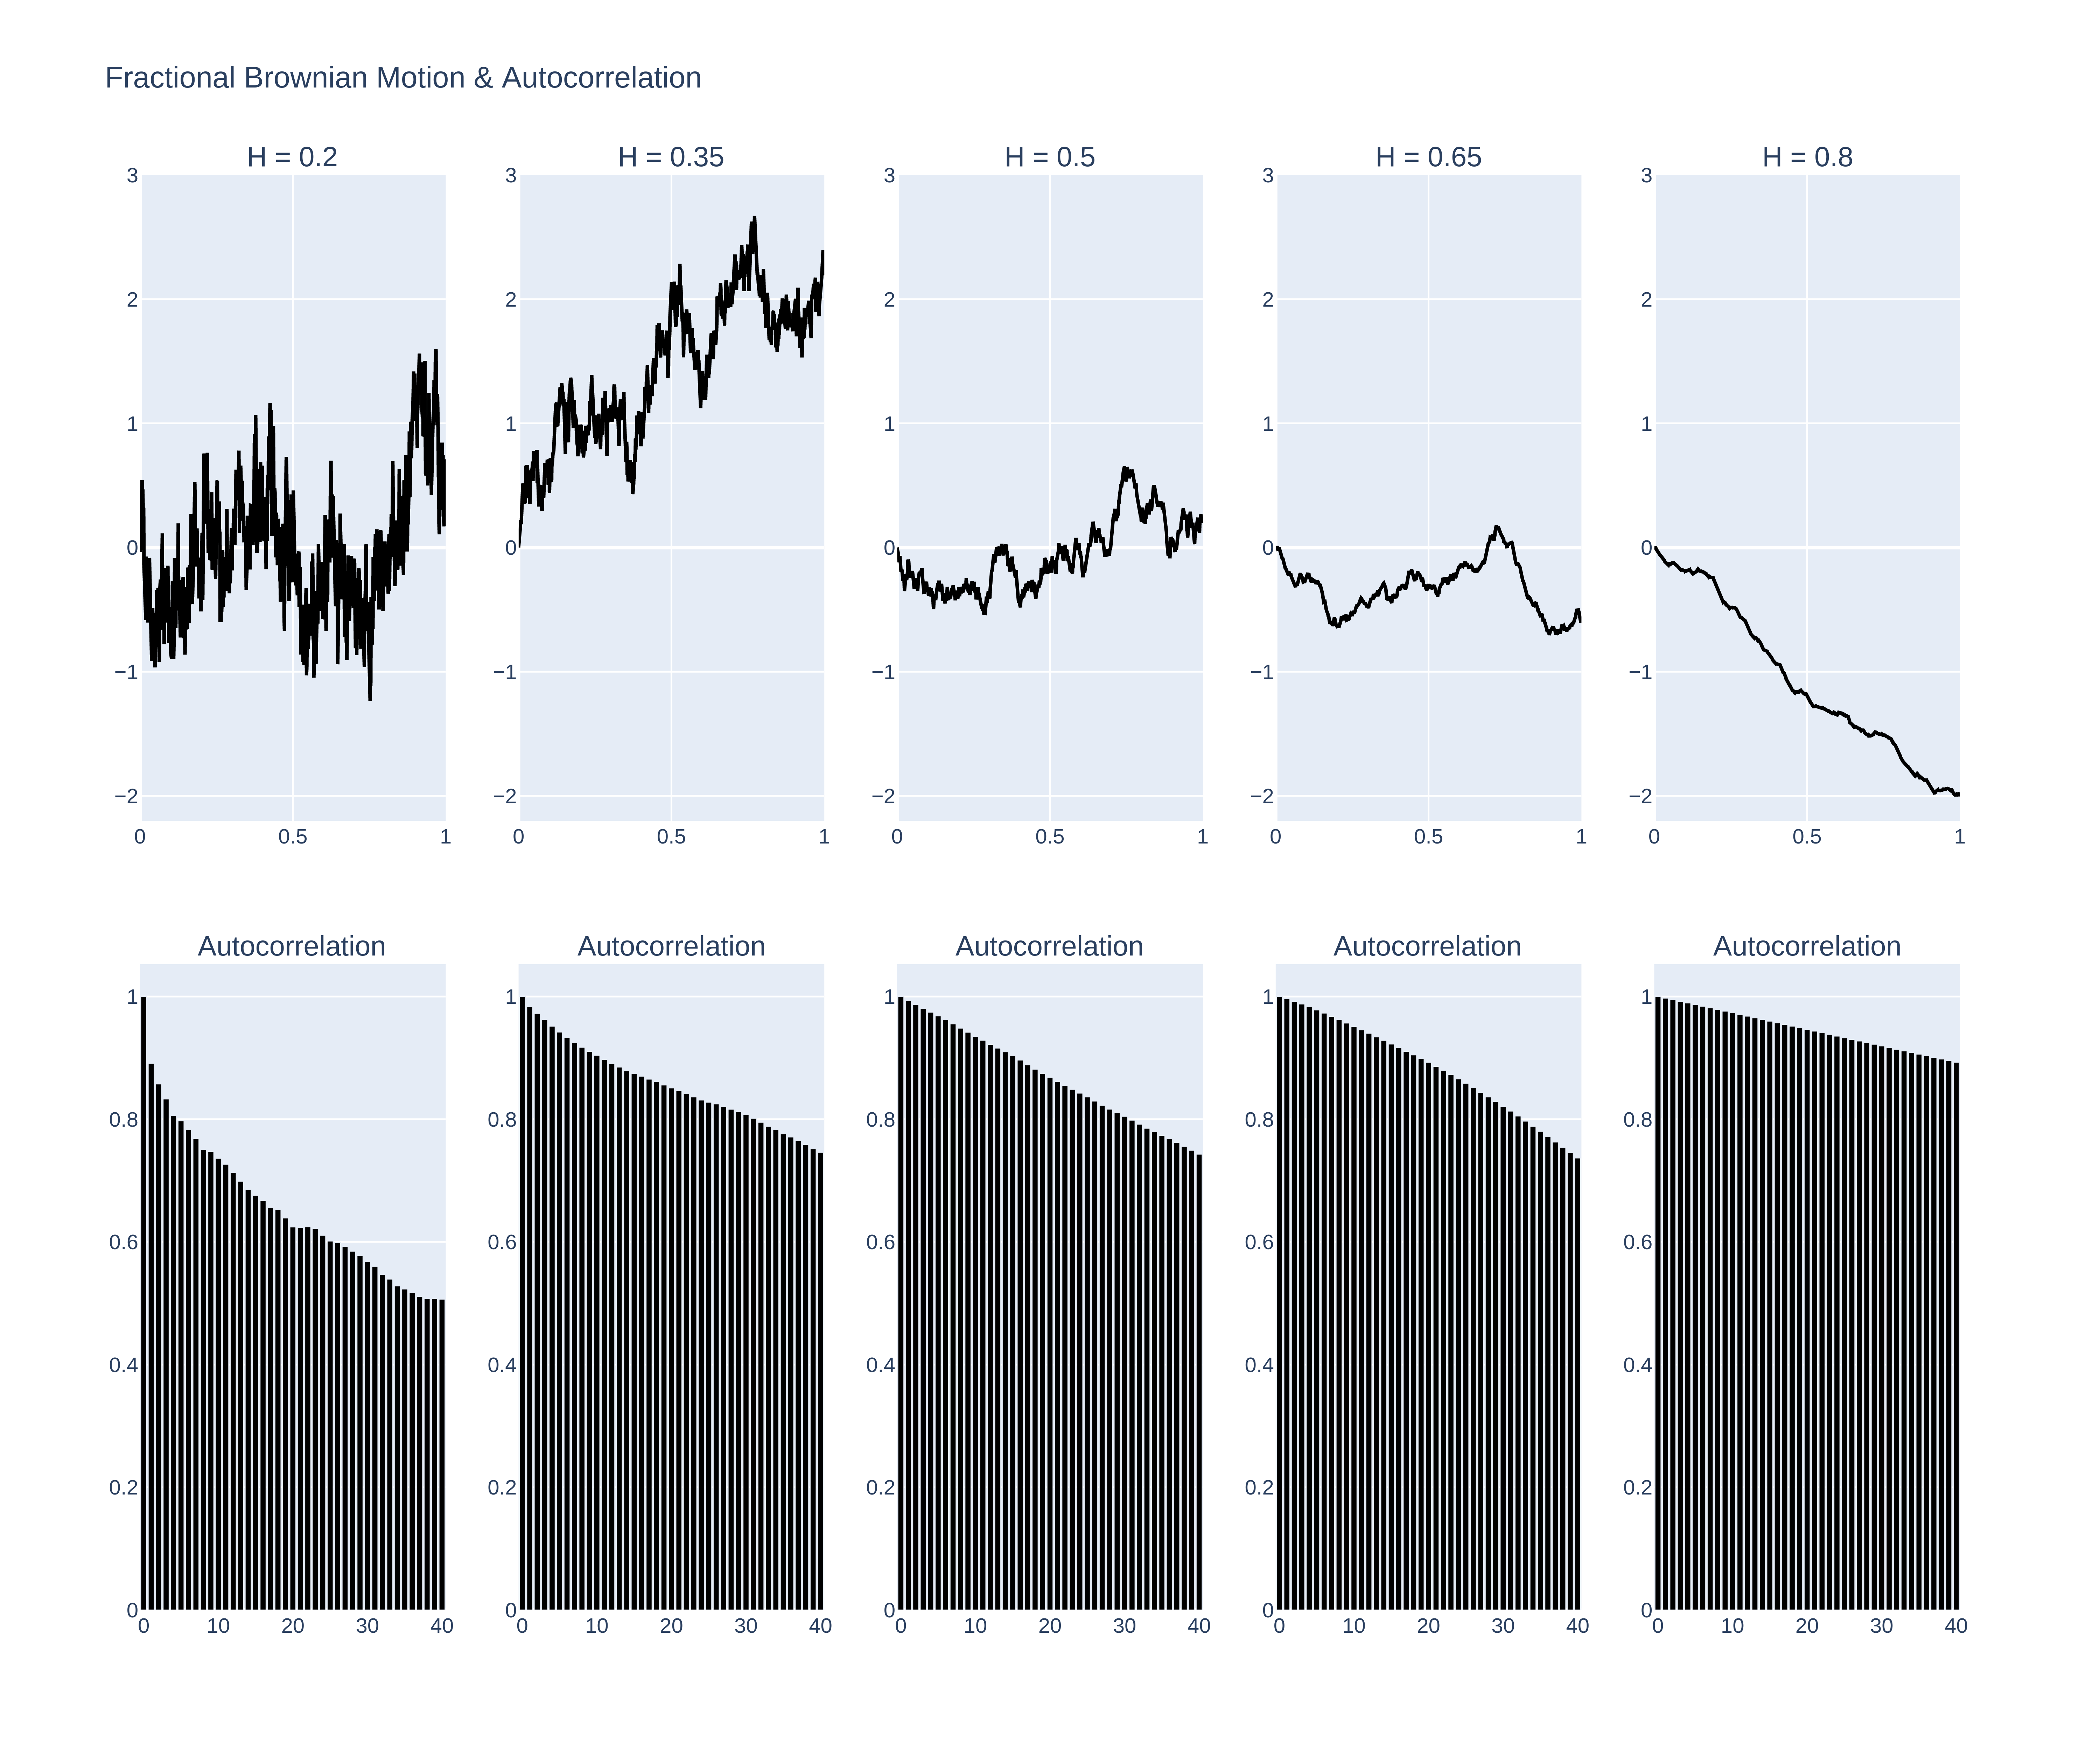
\includegraphics[width=0.8\textwidth]{img/fdm_autocorr}
    \caption{Simulation of fractional Brownian motion with different Hurst exponent and its autocorrelation function.
    Value of H = 0.2, 0.35, 0.5, 0.65, 0.8 and 1000 points is simulated over a day.}
    \label{fig:fbm_autocorr}
\end{figure}

\FloatBarrier

The behavior of the fractional Brownian motion varies significantly with the Hurst exponent \( H \).

When \( H \) is small (close to 0), the fBm exhibits high local variability, resulting in a highly granular trajectory with frequent fluctuations. The autocorrelation of increments decays rapidly, indicating that future values are weakly influenced by past values. This suggests a short-memory process, similar to standard Brownian motion.

As \( H \) increases, the autocorrelation decays more slowly, meaning that past values have a more significant impact on future values. This introduces a form of long-term dependence, where the process exhibits persistent trends. Consequently, the fBm trajectory appears smoother, with larger coherent movements and fewer abrupt changes.

In summary, a lower \( H \) leads to a more irregular and noisy path, characteristic of short-memory processes, while a higher \( H \) results in a smoother trajectory with stronger persistence.

\subsection{R/S and Modified R/S Analysis}

The R/S (Rescaled Range) analysis, introduced by Hurst and developed in various works by Mandelbrot, is certainly the most well-known method for estimating the Hurst exponent \(H\). This statistic is defined as the range of the partial sums of deviations from the mean of a time series divided by its standard deviation. Consider a time series \(Y_t\), \(t = 1, \dots, T\), with mean \(\bar{Y}\). The range \(R\) is defined as:
\begin{equation}
    R = \max_{1 \leq j \leq T} \left( Y_j - \bar{Y} \right) - \min_{1 \leq j \leq T} \left( Y_j - \bar{Y} \right).
\end{equation}

The R/S statistic is then computed by dividing the range by the standard deviation \(s_T\) of the series:
\begin{equation}
    Q_T = \frac{R}{s_T} = \frac{\max_{1 \leq j \leq T} \left( Y_j - \bar{Y} \right) - \min_{1 \leq j \leq T} \left( Y_j - \bar{Y} \right)}{s_T}, \quad \text{with } s_T = \sqrt{\frac{1}{T} \sum_{j=1}^{T} \left( Y_j - \bar{Y} \right)^2}.
\end{equation}

Empirical studies by Mandelbrot and Wallis (1969b) have shown that \(Q_T\) scales with the number of observations \(T\) according to
\begin{equation}
    Q_T \sim T^H,
\end{equation}
which implies that by taking logarithms, the Hurst exponent \(H\) can be obtained from
\begin{equation}
    H \sim \frac{\log(Q_T)}{\log(T)}.
\end{equation}

Unfortunately, the asymptotic distribution of the R/S statistic is not known, making it difficult to establish a
statistical test for the null hypothesis of short memory against the alternative hypothesis of long memory. Moreover,
the R/S statistic does not explicitly account for short-term autocorrelation in the data, which can inflate (or reduce)
the overall range and misrepresent the true variability of the series. Standard deviation estimates likewise ignore
autocorrelated structure over short horizons, compounding the bias.
As a result, the R/S measure can erroneously detect long memory when, in fact, short-term effects are responsible.
This shortfall motivated Lo’s Modified R/S procedure.

\subsection{Modified R/S Analysis}
\label{sec:modified_rs}

The modified R/S statistic, denoted by \(\tilde{Q}_T\), is defined as:
\begin{equation}
    \tilde{Q}_T = \frac{R}{\hat{\sigma}_T(q)},
\end{equation}
where
\begin{equation}
    \hat{\sigma}_T(q) = \sqrt{\frac{1}{T} \sum_{j=1}^{T} (Y_j - \bar{Y})^2 + \frac{2}{T} \sum_{j=1}^{T} w_j(q) \left[ \sum_{i=j+1}^{T} (Y_i - \bar{Y})(Y_{i-j} - \bar{Y}) \right]},
\end{equation}
and
\begin{equation}
    w_j(q) = 1 - \frac{j}{q + 1}.
\end{equation}

This statistic differs from the traditional R/S statistic only by its denominator. In the presence of autocorrelation,
the denominator does not solely represent the sum of the variances of the individual terms, but also includes
autocovariances weighted according to lags \(q\), with the weights \(w_j(q)\) suggested by Newey and West (1987).
Moreover, Andrews (1991) proposed a rule for choosing \(q\):
\begin{equation}
    q = \left[ k_T \right] \quad \text{where} \quad k_T = \left( \frac{3T}{2} \right)^{\frac{1}{3}} \left( \frac{2 \rho_1}{1 - \rho_1^2} \right)^{\frac{2}{3}},
\end{equation}
where \([k_T]\) is the integer part of \(k_T\), and \(\rho_1\) is the first-order autocorrelation coefficient.

Unlike the classical R/S analysis, the limiting distribution of the modified R/S statistic is known. The statistic \(V\), defined by
\begin{equation}
    V = \frac{\tilde{Q}_T}{\sqrt{T}},
\end{equation}
converges to the range of a Brownian bridge over the unit interval.
This convergence allows one to perform a statistical test for the null hypothesis of short memory against the
alternative hypothesis of long memory by referring to the critical value table provided by Lo (1991), shown in Table~\ref{table:critical_values}.
Therefore, accepting the null hypothesis implies that the series lacks the slow-decaying dependencies characteristic of long memory processes.

\subsection{Data}
\label{sec:data}

The data used in this analysis is monthly and consists of the historical closing prices of five major stock market indices: the S\&P 500,
Russell 2000, FTSE 100, Nikkei 225, and the DAX.
The data spans the period from September 10th, 1987, to February 28th, 2025.

For each index, the closing price time series was transformed using the natural logarithm to obtain a series of log returns.
Additionally, a stationarity test was conducted on the log return series using the Augmented Dickey-Fuller (ADF) test.
The results indicated that all series were non-stationary, suggesting the presence of unit roots.
To address this, the log returns were differenced once, after which they exhibited stationarity (test are available
in Table~\ref{table:adf_results}).

These differentiated log returns were then used to calculate the R/S and modified R/S statistics and estimate the Hurst exponent.
The purpose of using this data is to evaluate the long-term memory properties of financial markets, which can indicate persistence or mean-reversion in market behavior.



\subsection{Results}
\label{sec:results}

The following table summarizes the results of the R/S statistic, modified R/S statistic, and the estimated Hurst exponents for each of the five indices analyzed: \\

\begin{table}[h!]
    \centering
    \pgfplotstabletypeset[
        col sep=comma,
        header=true,
        string type,
        every head row/.style={before row=\hline, after row=\hline},
        every last row/.style={after row=\hline},
        columns/Ticker/.style={column name=Ticker, string type},
        columns/R/S Statistic/.style={column name=R/S Statistic, fixed, precision=2},
        columns/Hurst exponent (RS)/.style={column name=Hurst exponent (RS), fixed, precision=3},
        columns/modified Hurst exponent/.style={column name=modified Hurst exponent, fixed, precision=3},
        columns/critical value/.style={column name=critical value, fixed, precision=3},
        columns/long memory/.style={column name=long memory}
    ] {data/Hurst_results.csv}
    \caption{Results for R/S, Hurst exponent, modified Hurst exponent, critical value at 10\%, and rejection of the null
    hypothesis of long memory from 1987-09-10 to 2025-02-28. The Hurst exponent can be equal for the R/S and modified R/S methods in the case where
    the autocorrelation coefficients are less than zero (refer to Section~\ref{sec:long_range_dependence}), in this case we set $q$ equal to 0 and therefore the R/S and modified R/S share the same formula.}
    \label{tab:Hurst_results}
\end{table}

\FloatBarrier


Based on the results obtained from applying the traditional R/S method, all the series appear to exhibit long-term memory,
as the Hurst exponents are consistently greater than 0.5. However, the unknown asymptotic distribution of the traditional R/S
statistic prevents us from determining whether these Hurst values are statistically significant. To address this, we use the modified
R/S method, comparing the statistic \( V \) to the critical values provided by Lo (1991) (1.620 at the 10\% level and 1.747 at the 5\%
level in a one-tailed test). Our analysis shows that only one series the returns of the Russell 2000 small and mid cap (US) exhibits
statistically significant persistence, for the other series, despite Hurst exponents greater than 0.5, the null hypothesis of short memory cannot be rejected.

Since it seems unrealistic to characterize series with only one static Hurst exponent as the series might be influenced by local trends,
periods estimations, frequencies and to gain deeper insight into
the local scaling dynamics of these series, we now turn to Multifractal Detrended Fluctuation Analysis (MF-DFA).
Specifically, MF-DFA allows us to investigate the variety of local behaviors present in the time series by characterizing its multifractal
spectrum. This spectrum reveals how "rough" or "smooth" different segments of the series are and indicates the prevalence of each level of
irregularity. By examining the multifractal spectrum, we can determine whether the data exhibits a wide range of scaling behaviors, indicative
of multifractality, or if it behaves more uniformly. This transition to MF-DFA thus provides a complementary perspective that deepens our understanding
of the complex, scale-dependent dynamics governing the indices and how it relates to the dynamisms of the Hurst exponent.

\section{Multifractal Detrended Fluctuation Analysis}
\label{sec:mfdfa}

The Multifractal Detrended Fluctuation Analysis (MF-DFA) is a generalization of the standard Detrended Fluctuation
Analysis approach designed to detect multifractality in time series (Kantelhardt et al., 2002). The procedure can be summarized in five steps, as described below:

\begin{enumerate}
    \item \textbf{Profile construction.} Given a series \(\{x_k\}_{k=1}^N\), we first compute its mean \(\bar{x}\). Then, we build the profile
    \begin{equation}
        Z(i) \;=\; \sum_{k=1}^{i} \bigl(x_k \;-\; \bar{x}\bigr), \quad i \;=\; 1,2,\dots,N,
    \end{equation}
    where we use \(Z(i)\) instead of \(Y(i)\) to avoid confusion with previous definitions. This cumulative sum helps capture the local fluctuations in the data.

    \item \textbf{Division into segments.} We split the profile \(Z(i)\) into \(N_s \equiv \lfloor N/s \rfloor\) non-overlapping segments, each of length \(s\). Since \(N\) may not be a multiple of \(s\), we repeat this procedure starting from the opposite end, yielding a total of \(2N_s\) segments.

    \item \textbf{Detrending.} For each of the \(2N_s\) segments, we fit a polynomial trend (often linear or quadratic) and subtract it from \(Z(i)\) in that segment. Let \(z_\nu(i)\) be the fitting polynomial in segment \(\nu\). We then define the local variance as
    \begin{equation}
        F^2\bigl(s,\nu\bigr)
        \;=\;
        \frac{1}{s} \sum_{i=1}^s \Bigl[ Z\bigl((\nu-1)s + i\bigr) \;-\; z_\nu(i) \Bigr]^2.
    \end{equation}
    This detrending step removes possible polynomial trends in the data.

    \item \textbf{Generalized fluctuation function.} For each scale \(s\), we compute the \(q\)th-order fluctuation function,
    \begin{equation}
        F_q(s)
        \;=\;
        \left\{
          \frac{1}{2N_s} \sum_{\nu=1}^{2N_s} \Bigl[ F^2\bigl(s,\nu\bigr) \Bigr]^{q/2}
        \right\}^{1/q}.
    \end{equation}
    Varying \(q\) allows us to emphasize large (\(q>0\)) or small (\(q<0\)) fluctuations.

    In the special case \(q=0\), the fluctuation function is defined by a logarithmic averaging (see proof in Appendix Section~\ref{sec:proof_F0}):
    \begin{equation}
        F_0(s) = \exp\left(\frac{1}{4N_s} \sum_{\nu=1}^{2N_s} \ln\Bigl[F^2\bigl(s,\nu\bigr)\Bigr]\right).
    \end{equation}


    \item \textbf{Scaling behavior.} Finally, on double-logarithmic axes, we examine the dependence of \(F_q(s)\) on \(s\). If
    \begin{equation}
        F_q(s) \;\sim\; s^{h(q)},
    \end{equation}
    then \(h(q)\) is called the generalized Hurst exponent. In a multifractal series, \(h(q)\) varies with \(q\),
    indicating different scaling behaviors for large versus small fluctuations.
\end{enumerate}

For monofractal series, \(h(q)\) is approximately constant for all \(q\). In contrast, for multifractal
series, \(h(q)\) strongly depends on \(q\), revealing heterogeneity in the scaling of fluctuations.
For a graphical representation of the steps used in the MF-DFA, refer to Figure~\ref{fig:cumulative_profile_segment_partitioning}.

\subsection{Generalized Hurst Exponent}
\label{subsec:gen_hurst}

The S\&P 500 and Russell 2000 are ideal candidates for multifractal analysis.
The modified R/S statistic (M-R/S) for the S\&P 500 is approximately 0.501 very close to 0.5 which suggests that its
dynamics are consistent with efficient market behavior. In contrast, the Russell 2000 has a modified Hurst exponent of
approximately 0.588, indicating significant long-range dependencies and a less efficient market. Moreover, it is interesting
to observe that, in the graphical analysis (refer to Figure~\ref{fig:cumulative_returns}), there are periods when the Russell 2000
displays bullish trends while the S\&P 500 remains relatively flat for no apparent reason.

These discrepancies between the two series highlight their distinct scaling properties and market efficiencies. Our aim with
the multifractal analysis is to capture and quantify these differences in local scaling behavior. By analyzing the multifractal spectrum
of each index, we hope to match these structural discrepancies, thereby providing deeper insights into the dynamics of each market.
By analyzing both the S\&P 500 and Russell 2000, we gain insight into how differences in efficiency and persistence
affect their multifractal characteristics, thereby allowing us to exploit these structural differences in our trading strategy.
For this analysis, we will use the daily returns of the Russell 2000 index, S\&P 500 index from September 10th, 1987, to February 28th, 2025 (about 10 000 data points).

\begin{figure}[htbp]
    \centering
    \begin{tikzpicture}
        \begin{axis}[
            width=0.8\textwidth,
            height=6cm,
            xlabel={$q$},
            ylabel={$h(q)$},
            grid=major,
            legend style={
            font=\footnotesize,
            at={(0.5,-0.25)},
            anchor=north,
            legend columns=3
            }
        ]
            \addplot[
                blue,
                thick,
                mark=*,
                mark size=1.5pt
            ]
            table[
                x=q,
                y=h(q),
                col sep=comma
            ]
            {data/multifractal_spectrum_daily_Russell 2000.csv};
            \legend{Multifractal Spectrum}
        \end{axis}
    \end{tikzpicture}
    \caption{Multifractal Spectrum $h(q)$ for the Russell 2000 returns. Values of q are equally spaced between -3 and 3.
    The scale used are logly spaced between 10 and 500.}
\end{figure}

\FloatBarrier


If we take a closer look at the results from MF-DFA, we observe that the generalized Hurst exponent, $h(q)$,
varies as a function of q. The decrease sloping is a sign that the serie might exhibit multifractal behavior.
In a monofractal process, h(q) remains constant, reflecting uniform scaling.
Variation of h(q) with q indicates that small and large fluctuations scale differently.
The curvature of the line indicates the presence of heterogeneity in the distribution of singularities, with
different regions of the series characterized by varying degrees of irregularity.
Lower values of $q$ emphasize small fluctuations, while higher values highlight high fluctuations.
Therefore, this spectrum showcases that during periods of small fluctuations (q < 0) the series is likely to exhibit long-term
memory as the Hurst exponent is greater than 0.5, whether for drastic changes (q > 0) in the series behavior the Hurst exponent
is likely not to be high.
This result is consistent with our simulation of the fractional Brownian motion, where we can see that the
series exhibits smooth and regular behavior (calm fluctuations) for high Hurst exponent and sharply irregular behavior
(high fluctuations) for low Hurst exponent.


\begin{figure}[htbp]
    \centering
    \begin{tikzpicture}
        \begin{axis}[
            width=0.8\textwidth,
            height=6cm,
            xlabel={$q$},
            ylabel={$h(q)$},
            grid=major,
            legend style={
            font=\footnotesize,
            at={(0.5,-0.25)},
            anchor=north,
            legend columns=3
            }
        ]
            \addplot[
                blue,
                thick,
                mark=*,
                mark size=1.5pt
            ]
            table[
                x=q,
                y=h(q),
                col sep=comma
            ]
            {data/multifractal_spectrum_daily_SP500.csv};
            \legend{Multifractal Spectrum}
        \end{axis}
    \end{tikzpicture}
    \caption{Multifractal Spectrum $h(q)$ for the S\&P 500 returns. Values of q are equally spaced between -3 and 3.
    The scale used are logly spaced between 10 and 500.}
\end{figure}

\FloatBarrier

The multifractal spectrum for the S\&P 500 returns exhibits a similar behavior to that of the Russell 2000 returns,
except that it is less pronounced. At q = -3, the series exhibits a Hurst exponent of 0.56 compared to 0.65 for the
Russell 2000, those series seems to slightly differs in their behavior.
This difference, albeit modest, may hint at distinct market microstructure characteristics between the two indices.
For instance, the S\&P 500, with its larger and more liquid companies, might experience a smoothing effect on return
dynamics that could reduce the observable multifractality. In contrast, the Russell 2000, representing smaller-cap
stocks, may be subject to greater fluctuations and market inefficiencies, which could amplify multifractal behavior.
However, these interpretations remain speculative given the sensitivity of the multifractal analysis to the chosen
parameters and evaluation period.
Overall, our findings provide an interesting perspective on market behavior, suggesting that although both indices
share similar multifractal characteristics, subtle variations exist that could reflect underlying market differences.

From the MF-DFA analysis, we can also compute the Hölder exponent and multifractal spectrum.
Calculating the Hölder exponent and multifractal spectrum extends MF-DFA by detailing local behavior.
This logical continuation deepens insights into the complex, heterogeneous dynamics of the market.



\subsection{Hölder exponent}
The Hölder exponent $\alpha(q)$ characterizes the local multifractal strength of a signal and is obtained using the Legendre transform of $h(q)$:
\begin{equation}
\alpha(q) = h(q) + q h'(q).
\end{equation}
where $h'(q)$ is the derivative of $h(q)$ with respect to $q$. This exponent quantifies the intensity of local
singularities: lower values of $\alpha$ indicate highly irregular (or sharply singular) behavior, while higher
values correspond to smoother regions of the signal. Thus, the Hölder exponent reveals the heterogeneity of fluctuations within the signal.
This exponent describes the degree of multifractal in different parts of the series, revealing the heterogeneity of fluctuations.

\subsection{Multifractal Spectrum}
The multifractal spectrum $f(\alpha)$ provides a measure of the fractal dimension of subsets characterized by a given $\alpha$:
\begin{equation}
f(\alpha) = q [\alpha(q) - h(q)] + 1.
\end{equation}
This spectrum describes the distribution of singularities in the time series. A wider spectrum indicates stronger multifractality.

The analysis using the Hölder exponent and multifractal spectrum is a powerful tool for studying complex systems.
In particular, it enables one to identify and quantify regions of strong multifractal, which may correspond to extreme
events or sudden changes in dynamics and to describe the distribution and frequency of irregular behaviors in time series.
Thus, the multifractal approach offers a detailed and nuanced description of a signal's local variability, providing
essential insights for understanding and predicting its underlying dynamics. \\

We can distinguish two main contributions to the multifractal spectrum:
\[
\mathcal{M}(q) \propto
\underbrace{f_{\text{tail}}(q)}_{\substack{\text{Strongly non-Gaussian} \\ \text{distribution}}}
+
\underbrace{f_{\text{corr}}(q)}_{\substack{\text{Temporal correlations} \\ \text{in the series}}}
\]

Therefore, in the literature, the multifractality is often reffered as two types :

Type I multifractality arises
from a broad probability density function of the series values Jan W. Kantelhardt (2002) and al whereas Type II
multifractality stems from long-range correlations within the time series. This distinction enables us to identify and quantify
the type of multifractality present. By shuffling the series, we effectively eliminate the long-range correlations,
retaining only the influence of the value distribution. In an ideal monofractal series, the Hölder exponent would peak
at 0.5 thus, the difference between the exponents of the original and shuffled series reflects the contribution of
long-range correlations to the multifractality.


\begin{figure}[htbp]
    \centering
    \begin{tikzpicture}
        \begin{axis}[
            width=0.8\textwidth,
            height=6cm,
            xlabel={$\alpha$},
            ylabel={$f(\alpha)$},
            grid=major,
            legend style={
                font=\footnotesize,
                at={(0.5,-0.2)},
                anchor=north,
                legend columns=2
            }
        ]
            % Draw the multifractal spectrum of the shuffled signal (in red)
            \addplot[
                red,
                thick,
                mark=square*,
                mark size=1.5pt
            ]
            table[
                x=alpha_shuf,
                y=f_alpha_shuf,
                col sep=comma
            ]
            {data/f_alpha_alpha_russell 2000.csv};

            % Draw the multifractal spectrum of the original signal (in blue)
            \addplot[
                blue,
                thick,
                mark=*,
                mark size=1.5pt
            ]
            table[
                x=alpha,
                y=f_alpha,
                col sep=comma
            ]
            {data/f_alpha_alpha_russell 2000.csv};

            \legend{Shuffle, Original}
        \end{axis}
    \end{tikzpicture}
    \caption{Multifractal spectrum $f(\alpha)$ for the Russell 2000 returns.}
\end{figure}

\FloatBarrier

The multifractal spectrum $f(\alpha)$ for the Russell 2000 returns exhibits a bell-shaped curve,
indicating multiple scaling behaviors in the data. The peak near the center represents the most common local Hölder
exponent, while the spread around this peak highlights the diversity of singularities present in the series. A wider
spectrum suggests stronger multifractality, reflecting volatility clustering across multiple timescales and signaling diversified
behavior. Furthermore,
the approximate symmetry of the curve around its maximum implies that both large and small fluctuations are represented,
albeit with varying intensity. Overall, this bell-shaped spectrum underscores the complex, multi-scale nature of the
Russell 2000 returns.
A peak of the multifractal spectrum at $\alpha \approx 0.55$ indicates that the most common local Hölder exponent
in the Russell 2000 returns is around 0.55. In general, $\alpha > 0.5$ suggests a certain degree of persistence or
short to medium term correlation, $\alpha = 0.5$ aligns with a standard Brownian motion (random walk),
and $\alpha < 0.5$ signifies anti-persistence or more erratic behavior. Thus, an exponent of 0.55 may implies a
moderately rough signal neither purely random nor overly smooth highlighting the presence of multifractal characteristics.
Comparing it with the shuffle series, we observe that the $\alpha$ peak is lower than the original series, indicating that the
shuffled series exhibits a more uniform behavior. This suggests that the multifractality in the original series is primarily
driven by long-range correlations, while the shuffled series lacks this structure. It is still higher than 0.5, indicating
that the series is still multifractal but only because of the non-gaussian nature of returns (Kurtosis is 12.71). Moreover, the width spectrum
is approximately 0.2, in a random walk the width of the spectrum would be close to 0.1 (refer to Lukasz Czarnecki, Dariusz Grech 2009),
indicating that when shuffling the series, it behaves more like a random walk suggesting market efficiency.



\begin{figure}[htbp]
    \centering
    \begin{tikzpicture}
        \begin{axis}[
            width=0.8\textwidth,
            height=6cm,
            xlabel={$\alpha$},
            ylabel={$f(\alpha)$},
            grid=major,
            legend style={
                font=\footnotesize,
                at={(0.5,-0.2)},
                anchor=north,
                legend columns=2
            }
        ]
            % Draw the multifractal spectrum of the shuffled signal (in red)
            \addplot[
                red,
                thick,
                mark=square*,
                mark size=1.5pt
            ]
            table[
                x=alpha_shuf,
                y=f_alpha_shuf,
                col sep=comma
            ]
            {data/f_alpha_alpha_SP500.csv};

            % Draw the multifractal spectrum of the original signal (in blue)
            \addplot[
                blue,
                thick,
                mark=*,
                mark size=1.5pt
            ]
            table[
                x=alpha,
                y=f_alpha,
                col sep=comma
            ]
            {data/f_alpha_alpha_SP500.csv};

            \legend{Shuffle, Original}
        \end{axis}
    \end{tikzpicture}
    \caption{Multifractal spectrum $f(\alpha)$ for S\&P 500 returns.}
\end{figure}

\FloatBarrier

The multifractal spectrum $f(\alpha)$ for the S\&P 500 returns exhibits a different curve shortened on the right side.
The spectrum is narrower (0.27 between the maximum and minimum) compared to the Russell 2000 (0.4),
suggesting a possibly weaker multifractal nature, the difference between alpha min and alpha max is lower than the Russell 2000 ones
therefore it implies that the S\&P 500 returns exhibit a more uniform behavior compared to the Russell 2000. Let's recall that for
a random walk the alpha pic would be close to 0.5 and the spectrum width narrow.
The peak near the center for the original series is around 0.486. This may imply that the S\&P 500 returns exhibit a more stable
behavior compared to the Russell 2000, with less pronounced volatility clustering across multiple timescales.
The fact that the curve is shortened on the right but stretches deeper on the left means that the market exhibits fewer
ultra-calm intervals in favor of a greater propensity for abrupt or extreme fluctuations otherwise saying that this series
exhibit fatter tails.
Interestingly, the peak of the shuffled series is higher than the original one (0.53). Let's recall that from our analysis
with M-R/S, the S\&P 500 had a Hurst exponent of 0.501
,indicating that the series is likely to be a random walk. Moreover, the $\alpha$ peak of the original series is close to 0.5 (0.486)
reinforcing our first result via Hurst.
For both series, the width of the spectrum is approximately 0.27, if you look back at the Russell 2000, the width of the spectrum
shrinks to 0.2 when shuffling the series, indicating that the multifractality is primarily driven by long-range correlations.
In this spectrum, there is no long term correlation, the multifractality is only due to the non-gaussian nature of returns.
In the original returns, large jumps cluster together, creating many consecutive “rough” segments with low Hölder exponents.
Shuffling breaks up these clusters, so extreme returns become isolated among calmer data.
This reduces the frequency of very low h(t) and increases the share of intermediate h(t).
As a result, the modal Hölder exponent shifts upward even though the overall width remains unchanged. Shuffling the
series repeatedly won’t narrow the spectrum’s width; instead, it produces different modal $\alpha$ values simply because
the returns are randomly redistributed. \\


\begin{figure}[htbp]
    \centering
    \begin{tikzpicture}
        \begin{axis}[
            width=0.8\textwidth,
            height=6cm,
            xlabel={$\alpha$},
            ylabel={$f(\alpha)$},
            grid=major,
            legend style={
                font=\footnotesize,
                at={(0.5,-0.2)},
                anchor=north,
                legend columns=2,
            },
        legend cell align=center
        ]
            % Draw the multifractal spectrum of the shuffled signal (in red)
            \addplot[
                red,
                thick,
                mark=square*,
                mark size=1.5pt
            ]
            table[
                x=alpha,
                y=f_alpha,
                col sep=comma
            ]
            {data/f_alpha_alpha_SP500.csv};

            % Draw the multifractal spectrum of the original signal (in blue)
            \addplot[
                blue,
                thick,
                mark=*,
                mark size=1.5pt
            ]
            table[
                x=alpha,
                y=f_alpha,
                col sep=comma
            ]
            {data/f_alpha_alpha_Russell 2000.csv};

        \addplot[
                yellow,
                thick,
                mark=*,
                mark size=1.5pt
            ]
            table[
                x=alpha,
                y=f_alpha,
                col sep=comma
            ]
            {data/f_alpha_alpha_random_walk.csv};



            \legend{SP500, Russell, Random Walk}
        \end{axis}
    \end{tikzpicture}
    \caption{Comparision of multifractal spectrum for SP500, Russell 2000 and a random walk.}
\end{figure}

\FloatBarrier

From this analysis, we can conclude that the S\&P 500 returns exhibit a behavior close to the one of a random walk and
that it's multifractality comes from the non-gaussian nature of the returns (Kurtosis is estimated 28.41) since the width
of the spectrum doesn't change much with the shuffling series. Whereas for the Russell 2000 it clearly comes from the long-range
correlations (Kurtosis is estimated 12.71) since the width of the spectrum shrinks when shuffling the series.
Therefore, the inefficency could be measured by the width of the spectrum rather than the $\alpha$ peak of the series.

In an ideal random walk (i.i.d. Gaussian increments), the multifractal spectrum collapses to a single point its width
$\Delta \alpha$ is close to 0 because every local segment is statistically identical and fully unpredictable. By contrast, our
return series shows $\Delta \alpha$ >0, revealing multiple coexisting dynamics (calm trends, sudden shocks, reversals).
This width therefore quantifies market inefficiency: the larger $\Delta \alpha$ is, the more the series departs from pure randomness
and the more distinct local regimes it contains.



\subsection{Proposition of an Inefficiency Index}

To capture market inefficiency, we propose combining two key structural components:

\begin{enumerate}
    \item \textbf{Fractal Difference:}\\[1ex]
    The width of the multifractal spectrum is defined as
    \begin{equation}
    \Delta \alpha = \alpha_{\text{max}} - \alpha_{\text{min}},
    \end{equation}
    where $\alpha$ is the singularity exponent obtained via an MF-DFA analysis.

    \item \textbf{Deviation of the Rolling Hurst:}\\[1ex]
    In an efficient market (i.e., following a Brownian motion) the Hurst exponent is expected to be
    \begin{equation}
    H = 0.5.
    \end{equation}
    Therefore, the deviation is measured by
    \begin{equation}
    \left|H_{\text{rolling}} - 0.5\right|.
    \end{equation}
\end{enumerate}

We define the inefficiency index $I$ as
\begin{equation}
I = \Delta\alpha_{\text{diff}} \times \left|H_{\text{rolling}} - 0.5\right|,
\end{equation}
where $\Delta\alpha_{\text{diff}}$ is the absolute difference between the multifractal spectrum widths of two indices (for example, S\&P 500 versus Russell 2000).
It gives us insights on which market seems to be more inefficient.


An efficient market should exhibit
\begin{equation}
H = 0.5,
\end{equation}
so any deviation quantified by $\left|H_{\text{rolling}} - 0.5\right|$ indicates the presence of temporal correlations:
\begin{itemize}
    \item $H>0.5$ signals persistence (trends are likely to continue),
    \item $H<0.5$ signals anti-persistence (a tendency for mean reversion).
\end{itemize}

A larger $\Delta \alpha$ indicates significant variability in local scaling behaviors,
meaning that the market exhibits a more complex structure and may be less efficient. By
combining both the fractal difference and the deviation of $H$ from 0.5, the inefficiency index $I$
captures two complementary aspects of market inefficiency structural complexity and long-range memory deviation.
This combined signal serves as both a filtering criterion and an independent confirmation of inefficiency.



\section{Trading Strategy}

The strategy is based on the proposed Inefficiency Index, rolling modified Hurst and a momentum signal. It aims to exploit differences in the
long-term memory and multifractal characteristics between the Russell 2000 and S\&P 500 indices. The expectation is that
these structural differences, captured by deviations in the rolling Hurst exponent and the multifractal spectrum width,
reveal market inefficiencies that can be harnessed for trading.

First, we compute the difference in the log returns of the Russell 2000 index and the S\&P 500 index. A positive value
indicates that the S\&P 500 is outperforming the Russell 2000, while a negative value indicates the converse.

Next, we calculate a rolling Hurst exponent on this spread using the modified R/S statistic, which helps correct for
short-term autocorrelation bias over a six‐month window. In parallel, a rolling momentum indicator is derived from the
same spread by taking the mean of the past 220 days returns with a 20‐day shift to not take into account the last month.
We then construct the inefficiency index defined as
\[
I = \Delta\alpha_{\text{diff}} \times \left|H_{\text{rolling}} - 0.5\right|,
\]
where \(\Delta \alpha_{\text{diff}}\) represents the absolute difference between the multifractal spectrum widths of the two
indices. It is computed as a rolling window of 4 years since in provides the best compromise between significance of the results
and number of data points required.

Starting with an equal-weighted portfolio (50\% in the Russell 2000 and 50\% in the S\&P 500), the positions are adjusted as follows:

\begin{itemize}
    \item If the rolling Hurst exponent is greater than 0.5, the momentum is positive (indicating that the S\&P 500 is
    outperforming the Russell 2000), and if the inefficiency is positive,
    then the spectrum width ($\alpha$max - $\alpha$min) of the S\&P 500 is larger than that of the Russell 2000. This implies that the S\&P 500 exhibits stronger
    persistence and a more complex fractal structure, suggesting inefficiency. In this case, we overweight the S\&P 500 by allocating
    80\% to it and 20\% to the Russell 2000.

    \item If the rolling Hurst exponent is greater than 0.5 and the momentum is negative (indicating that the Russell 2000 is
    outperforming the S\&P 500), if the inefficiency index is negative (meaning that the alpha width of the
    Russell 2000 is wider than that of the S\&P 500). Hence, we overweight the Russell 2000, assigning 80\% to it and 20\% to the S\&P 500.

    \item If the rolling Hurst exponent is below 0.5, implying no clear persistence, we maintain a neutral allocation (50\% in each index).
\end{itemize}


\begin{figure}[ht]
    \centering
    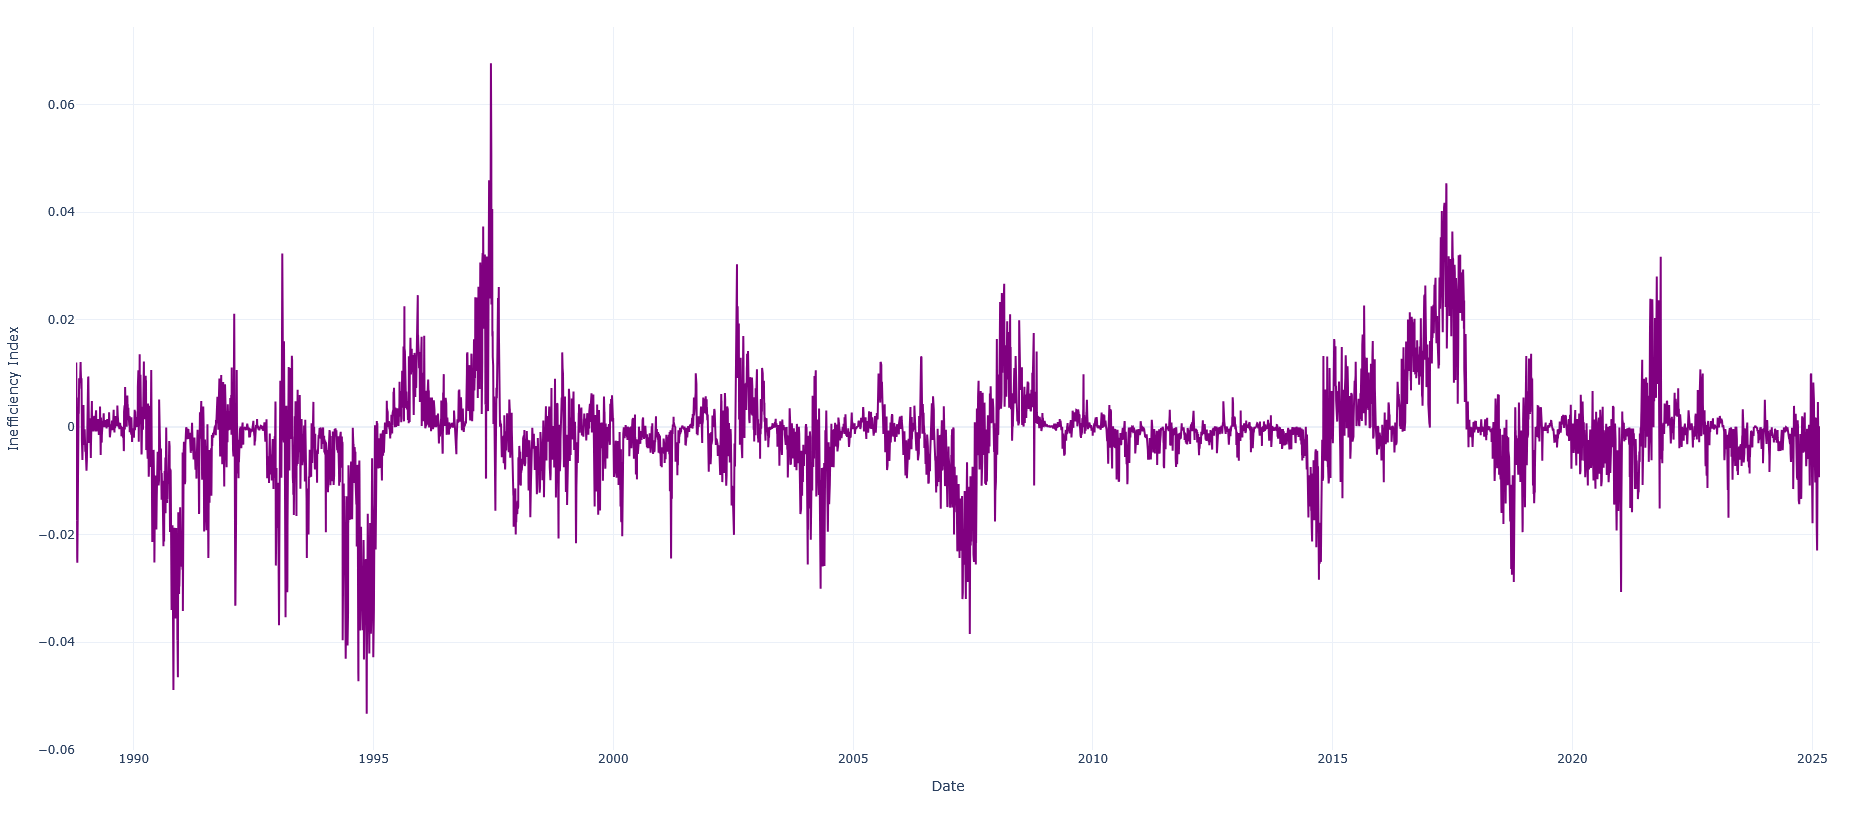
\includegraphics[width=0.8\textwidth]{img/inefficiency_index.png}
    \caption{Inefficiency index computed based on the difference between the spectrum width ($\alpha$max - $\alpha$min) between the
    S\&P 500 and Russell 2000, from 1991-11-15 to 2025-02-28. The window used here is 4 years as it provides the best compromise between significance of the results
    and number of data points required.}
    \label{fig:inefficiency_index}
\end{figure}
\FloatBarrier



\begin{figure}[ht]
    \centering
    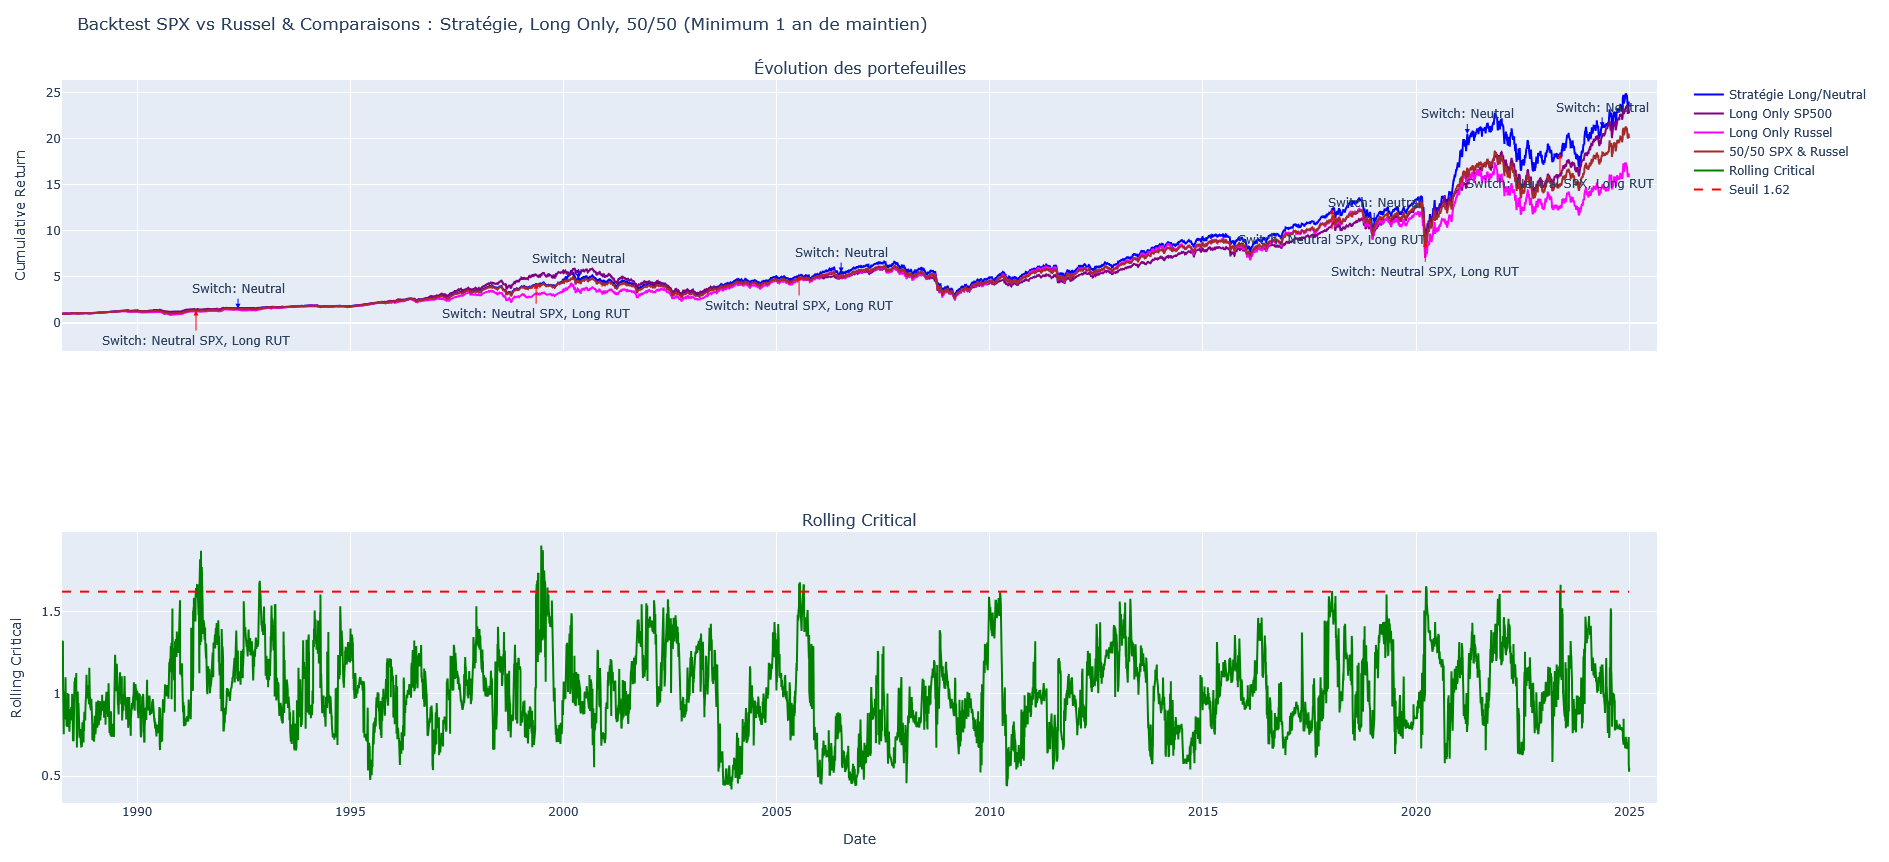
\includegraphics[width=0.8\textwidth]{img/backtest_long_neutral.png}
    \caption{Comparison of the performance of the ModifOverlap120 strategy (blue) with the 50/50 portfolio (black).
        The backtest period is from 1991-11-15 to 2025-02-28.}
    \label{fig:cumulative_performance}
\end{figure}

\FloatBarrier

\begin{table}[!h]
    \centering
    \pgfplotstabletypeset[
        columns={Strategy,Annualized Return,Annualized Volatility,Sharpe,Max Drawdown},
        columns/Strategy/.style={string type,column name=Strategy},
        columns/Annualized Return/.style={column name=Annualized Return},
        columns/Annualized Volatility/.style={column name=Annualized Volatility},
        columns/Sharpe/.style={column name=Sharpe},
        columns/Max Drawdown /.style={column name=Max Drawdown}
    ]{data/backtest_long_neutral_results.csv}
    \caption{Performance metrics of the strategies ModifOverlap120 (5 bps transaction fees) compared to 50/50 Russell/S\&P 500 portfolio
    from 1991-11-15 to 2025-02-28.}
    \label{tab:performance_table}
\end{table}

\FloatBarrier

\label{sec:backtest_results}
We tested severals strategies to see how robust the results are, the ModifOverlap120 correspond to the estimation of a
Hurst based modified R/S statistic using a rolling window of 120 days and the ModifOverlap120NoFilter corresponds to the estimation of a
Hurst based modified R/S statistic using a rolling window of 120 days without using the inefficiency index as a signal filter.
The results are shown in Table~\ref{tab:performance_table} and Figure~\ref{fig:cumulative_performance} (for a more detail analysis
on window size see Table~\ref{tab:performance_table_window_120}).
All the strategies outperform the 50/50 portfolio and the long only Russell 2000 portfolio. The portfolio composition and position switching
for the ModifOverlap120 can be seen in Figure~\ref{fig:position_switching}.
The ModifOverlap120 strategy outperforms the 50/50 portfolio in all metrics, except
that it achieves a slightly higher volatility over the period. The ModifOverlap120 and ModifOverlap120NoFilter strategies
shows similar results except that the use of the inefficency index as a filter improve the performance of the strategy by
achieving a lower max drawdown.


\section{Conclusion}

In this paper, we examined the long-term memory and multifractal properties of major stock market indices using both
traditional and modified R/S analysis alongside Multifractal Detrended Fluctuation Analysis (MF-DFA). Our findings
suggest that, while most series display Hurst exponents greater than 0.5 implying some degree of persistence the
modified R/S approach indicates that only the Russell 2000 exhibits statistically significant long memory.
In contrast, the S\&P 500 shows a more subdued multifractal behavior, with a narrower spectrum and lower extremal Hölder
exponents. This difference may reflect underlying market microstructure characteristics, such as liquidity and the size
of constituent companies, but these interpretations should be treated with caution. The Hurst exponent seems to be able
to capture differences in the multifractal spectrum between the two indices, with the Russell 2000 that appears to
display a broader spectrum and more distinct multifractal characteristics compared to the S\&P 500. Overall, the outperformance
of the strategies seems to hold depending on the window size used, and the proposed inefficiency brings value as a risk
limiting filter.

\section{Discussion}

It is important to emphasize that the methods used in our study both the static Hurst exponent and the multifractal
analysis are highly sensitive to the chosen data frequency, evaluation period, and potential structural breaks. The
apparent persistence observed in the Russell 2000, for instance, may be influenced by these factors, while the more
stable behavior seen in the S\&P 500 could result from its larger, more liquid market composition.

Overall, while our results provide an intriguing perspective on market dynamics and offer a foundation for a trading
strategy based on these multifractal measures, they should be interpreted with a degree of caution. Future research
should aim to extend this analysis to a broader set of assets (pair clustering) and refine the estimation techniques
to confirm the statistical significance of the observed multifractal effects.

\section{Appendix}

\subsection{Demonstration of the covariance of fractional Brownian motion (fBm)}
\label{sec:covariance_fbm}

The fractional Brownian motion (fBm), denoted by \( X_H(t) \), is defined as a zero-mean continuous-time Gaussian process whose increments are correlated. Its covariance function is given by:

\[
C_H(t,s) = \frac{\sigma^2}{2}\left(t^{2H}+s^{2H}-|t-s|^{2H}\right)
\]

where \( H \in (0,1) \) is the Hurst exponent.

A fractional Brownian motion \( X_H(t) \) with \( X_H(0)=0 \) has increments that are normally distributed with zero mean, specifically:

\[
X_H(t)-X_H(s) \sim \mathcal{N}(0,\sigma^2|t-s|^{2H})
\]

Given that the process is centered (zero mean), the covariance is defined as:

\[
C_H(t,s) = \text{Cov}(X_H(t), X_H(s)) = \mathbb{E}[X_H(t)X_H(s)]
\]

Using the following algebraic identity:

\[
X_H(t)X_H(s) = \frac{1}{2}\left[X_H(t)^2 + X_H(s)^2 - (X_H(t)-X_H(s))^2\right]
\]

the covariance becomes:

\[
C_H(t,s) = \frac{1}{2}\left(\mathbb{E}[X_H(t)^2]+\mathbb{E}[X_H(s)^2]-\mathbb{E}[(X_H(t)-X_H(s))^2]\right)
\]


We have by definition of fBm:

\[
\mathbb{E}[X_H(t)^2] = \sigma^2 t^{2H}, \quad \mathbb{E}[X_H(s)^2] = \sigma^2 s^{2H}, \quad \mathbb{E}[(X_H(t)-X_H(s))^2] = \sigma^2 |t-s|^{2H}
\]

Substituting these into our covariance expression, we get:

\[
C_H(t,s) = \frac{1}{2}\left(\sigma^2 t^{2H} + \sigma^2 s^{2H} - \sigma^2 |t-s|^{2H}\right)
\]


Factoring out the term \( \sigma^2 \), we arrive at the final covariance formula:

\[
\boxed{C_H(t,s) = \frac{\sigma^2}{2}\left(t^{2H} + s^{2H} - |t-s|^{2H}\right)}
\]

This covariance function entirely characterizes the dependence structure of fractional Brownian motion, revealing long-term correlation when \(H>0.5\) (persistence) and anti-correlation when \(H<0.5\) (anti-persistence).
To comeback where you left off, see Section~\ref{eq:fbm_covariance}. \\

\subsection{Critical Values for the Modified R/S Test}

The critical values for the modified R/S test are provided in the table below. These values are used to assess whether the series exhibits long memory behavior based on the modified R/S statistic.

\begin{table}[ht!]
\centering
\begin{tabular}{|c|c|c|}
\hline
\textbf{Significance Level} & \textbf{critical value (modified R/S Statistic)} \\
\hline
0.005 & 2.098\\
0.05 & 1.747\\
0.10 & 1.620\\

\hline
\end{tabular}
\caption{Critical values for the modified R/S Statistic (Lo, 1991). To come back where you left off, see Section~\ref{sec:modified_rs}}
    \label{table:critical_values}
\end{table}

\subsection{Definition (Time Domain)}
\label{sec:long_range_dependence}
A stationary process \(X_t\) is said to exhibit long‐range dependence (long memory) if there exist constants

\[
a\in(0,1),\quad c>0,
\]
such that its autocorrelation function \(\rho(k)\) satisfies

\begin{equation}
\lim_{k \to \infty}
\frac{\rho(k)}{c\,k^{-\alpha}}
=1
\end{equation}
where \(\rho(k)\) is the autocovariance function, \(c\) is a constant (V.Mignon 2003). To comeback where you left off,
see Section~\ref{sec:results}.



\begin{table}[h!]
    \centering
    \pgfplotstabletypeset[
        col sep=comma,
        header=true,
        string type,
        every head row/.style={before row=\hline, after row=\hline},
        every last row/.style={after row=\hline},
        columns/Ticker/.style={column name=Ticker, string type},
        columns/P-Value of log prices/.style={column name=P-Value of log Prices, fixed, precision=3},
        columns/P-Value of log differentiated return/.style={column name=P-Value of Log Differentiated Return, fixed, precision=3}
    ] {data/adf_results.csv}
    \caption{P-values from the Augmented Dickey-Fuller (ADF) test for stationarity. The P-value of log prices refers to the Augmented Dickey Fuller test (ADF) on log prices,
     while the P-value of log-differentiated prices indicates the ADF test on log-differentiated returns. The null hypothesis is non-stationarity.
    To come back where you left off, see Section~\ref{sec:data}}
    \label{table:adf_results}
\end{table}


\begin{figure}[ht]
    \centering
    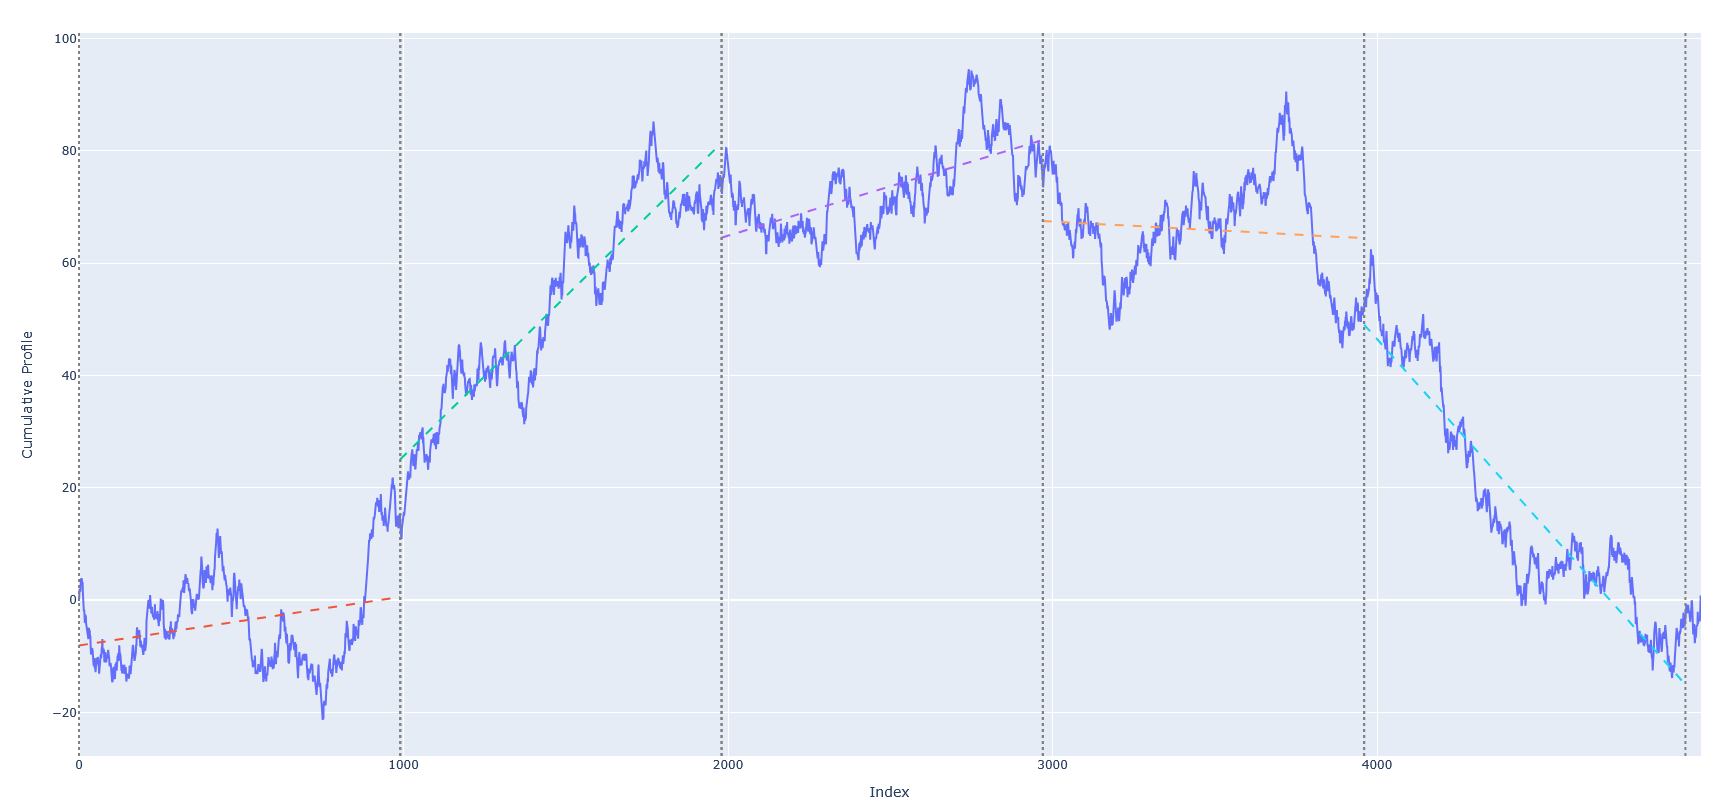
\includegraphics[width=0.8\textwidth]{img/cumulative_profile_segment_partitioning}
    \caption{Simulation of the MF-DFA steps, the series is the Russell 2000 returns
    split into segments of length 880 to represents the steps of MF-DFA.
        The blue line represents the cumulative sum of the centered returns, while the coloured lines represent the polynomial fit for
    each segment. To come back where you left off, see Section~\ref{sec:mfdfa}.}
    \label{fig:cumulative_profile_segment_partitioning}
\end{figure}
\FloatBarrier


\subsection{Proof of \(F_0(s)\) as \(q\to0\)}
\label{sec:proof_F0}
\begin{frame}{Proof of \(F_0(s)\) as \(q\to0\)}
  \[
    F_q(s)
    =\Bigl[\tfrac{1}{2N_s}\sum_{v=1}^{2N_s}\bigl(F_v^2(s)\bigr)^{\!q/2}\Bigr]^{1/q}
    \;\Longrightarrow\;
    \ln F_q(s)
    =\frac{1}{q}\ln S(q),
  \]
  where
  \[
    S(q)=\frac{1}{2N_s}\sum_{v=1}^{2N_s}e^{\tfrac{q}{2}\ln F_v^2(s)}.
  \]
  As \(q\to0\), \(\ln S(q)\to0\) and we apply L’Hôpital:
  \[
    \lim_{q\to0}\ln F_q(s)
    =\lim_{q\to0}\frac{\ln S(q)}{q}
    =\left.\frac{S'(q)}{S(q)}\right|_{q=0}
    =\frac{1}{4N_s}\sum_{v=1}^{2N_s}\ln F_v^2(s).
  \]
  Exponentiating:
  \[
    F_0(s)
    =\exp\!\Bigl[\tfrac{1}{4N_s}\sum_{v=1}^{2N_s}\ln F_v^2(s)\Bigr]
    =\exp\!\Bigl[\tfrac{1}{2N_s}\sum_{v=1}^{2N_s}\ln F_v(s)\Bigr].
  \]
  \vspace{4pt}
  \textit{Thus \(F_0(s)\) is the geometric mean of the segment fluctuations.}
    To comeback where you left off, see Section~\ref{sec:mfdfa}.
\end{frame}


\begin{figure}[ht]
    \centering
    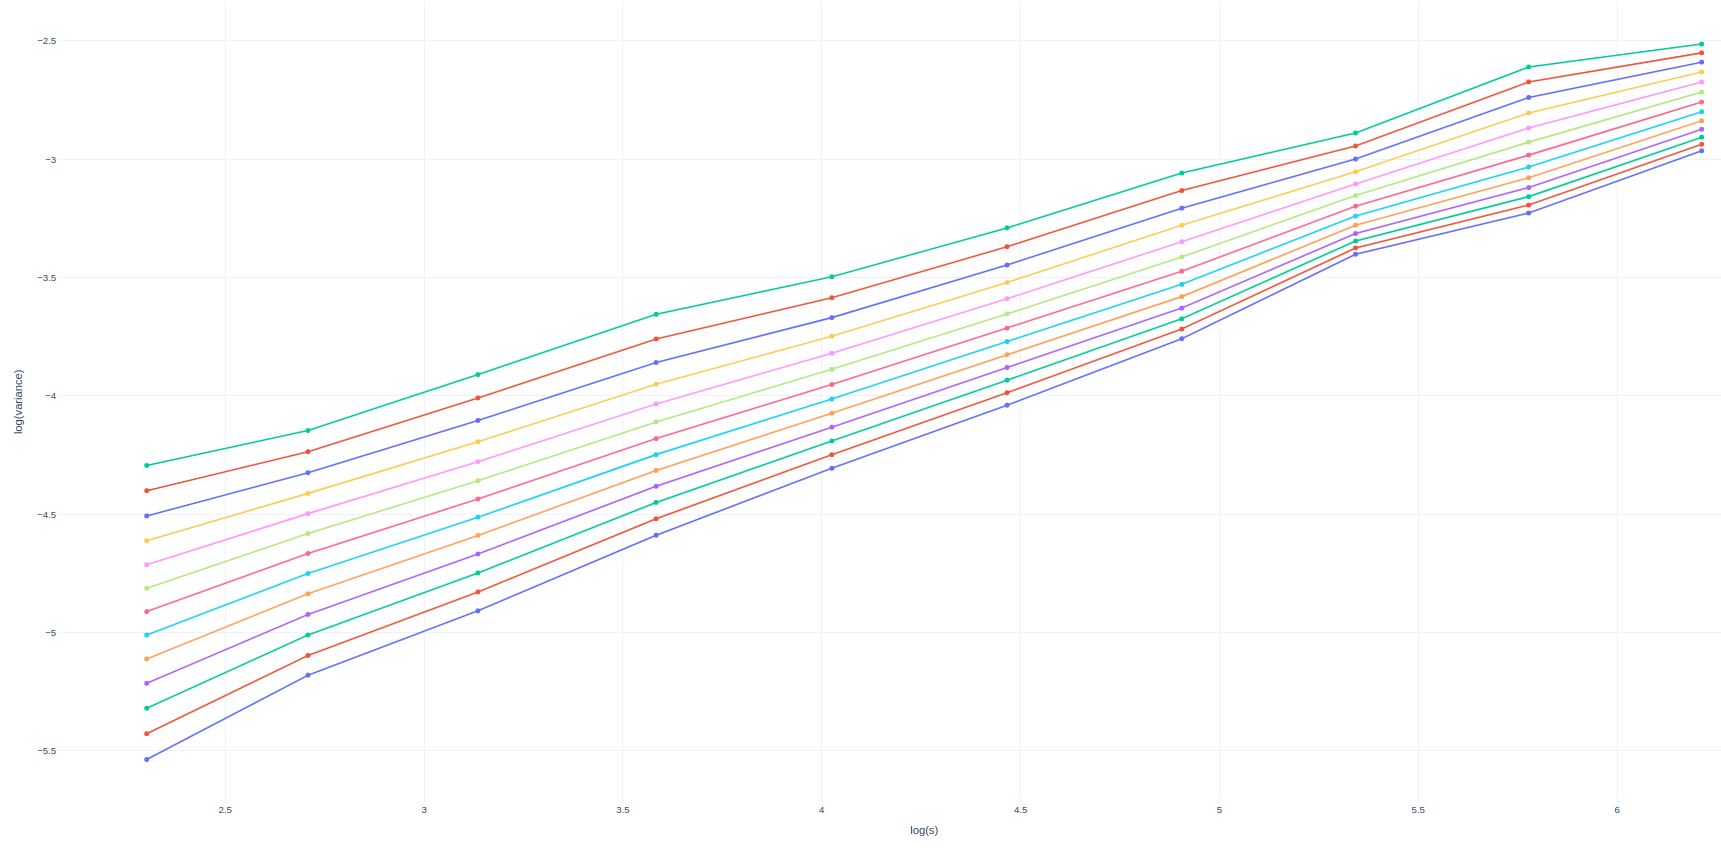
\includegraphics[width=0.8\textwidth]{img/log_variance_log_scale}
    \caption{Plot of the log scales (10 logly spaced increments from 10 to 500) against the log variance for each values of q, green line (highest line) represents q = -3
    the lowest line represents q = 3. The slope of the line is the Hurst exponent for each q.}
    \label{fig:log_variance_log_scale}
\end{figure}
\FloatBarrier

\begin{figure}[ht]
    \centering
    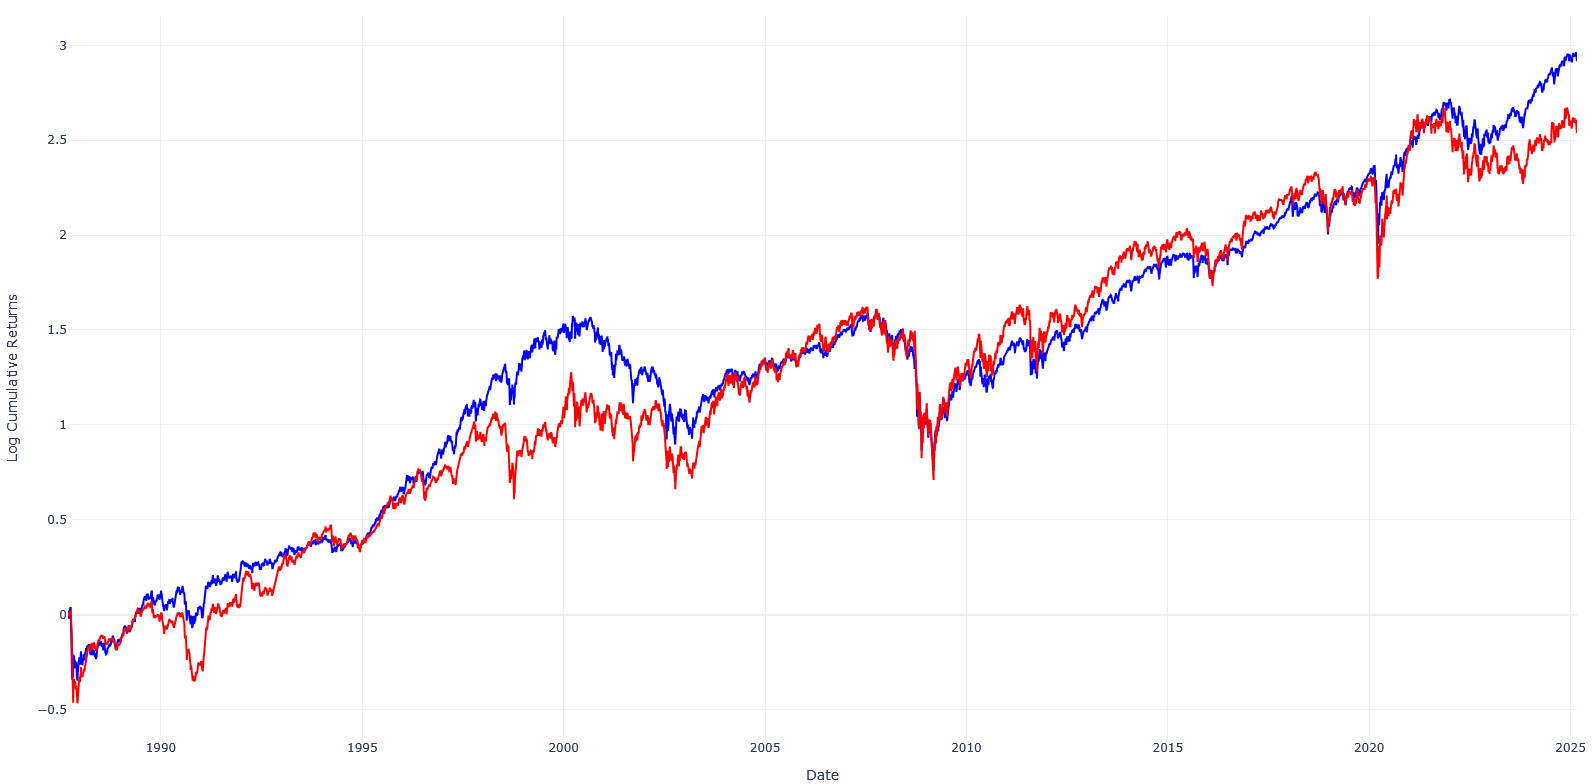
\includegraphics[width=0.8\textwidth]{img/log_cumulative_returns.png}
    \caption{Log cumulative returns of S\&P 500 (blue) and Russell 2000 (red) from 1987-09-11 to 2025-02-28.
    To come back where you left off, see Section~\ref{subsec:gen_hurst}.}
    \label{fig:cumulative_returns}
\end{figure}


\FloatBarrier


\begin{figure}[ht]
    \centering
    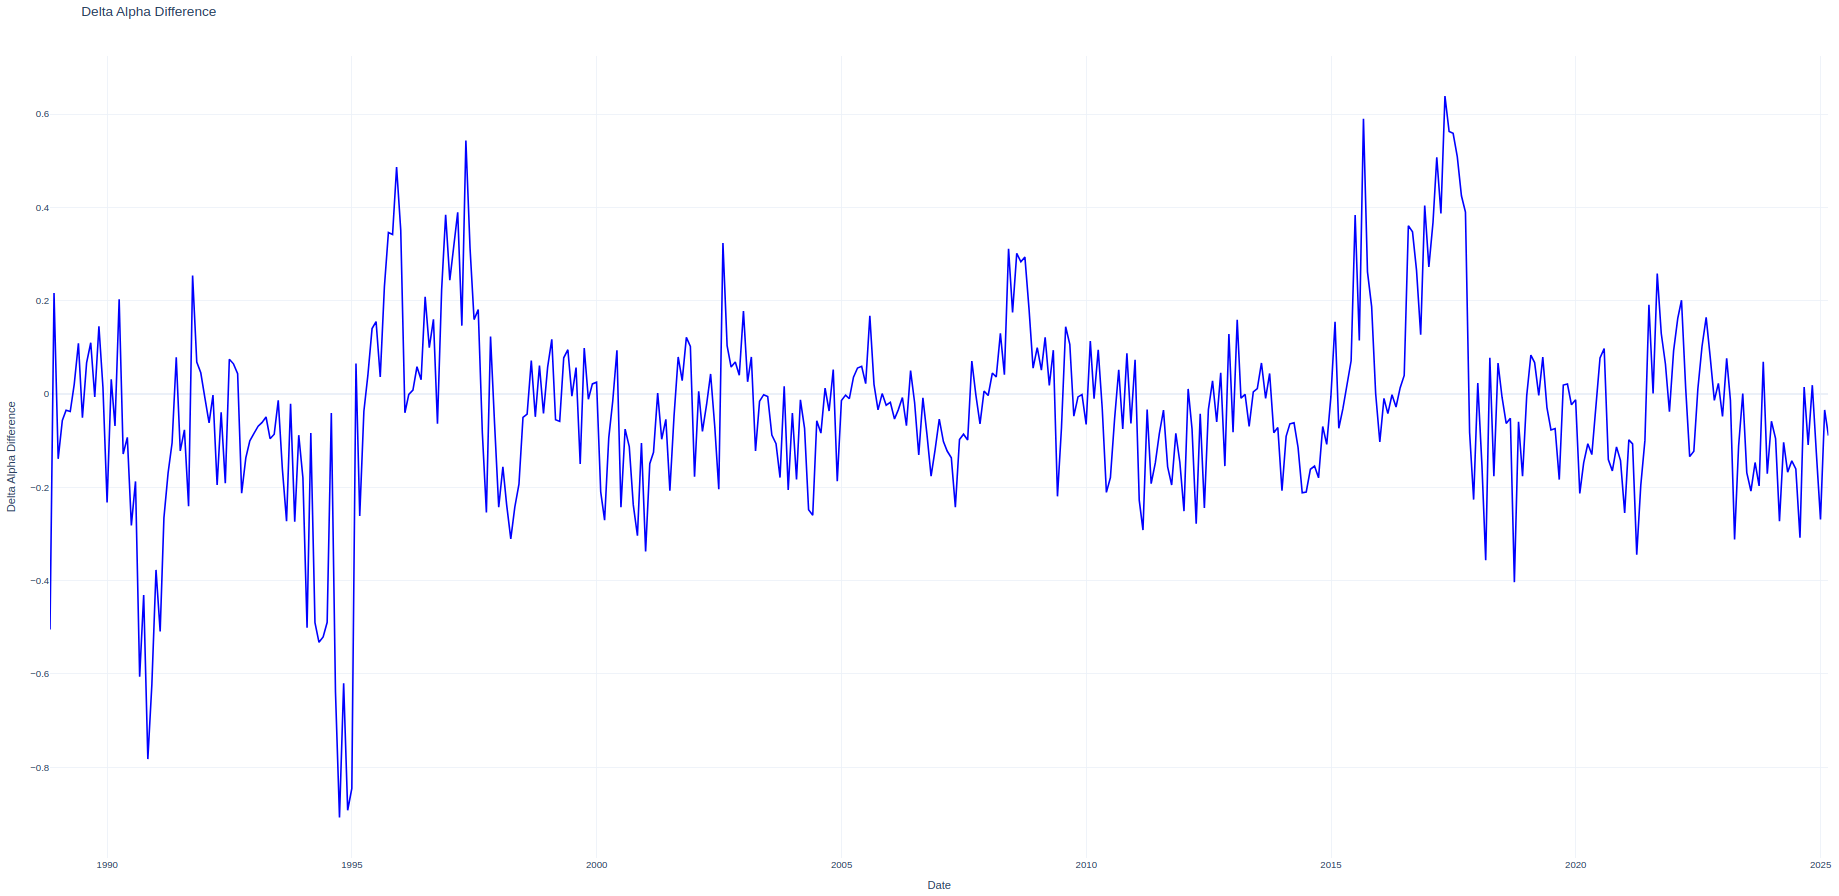
\includegraphics[width=0.8\textwidth]{img/delta_alpha_resample_m.png}
    \caption{Rolling alpha width difference computed with a rolling window of 1008 days (4 years)
        for the S\&P 500 and Russell 2000. The data in this example is resampled to monthly for better clarity.}
    \label{fig:rolling_alpha_width}
\end{figure}
\FloatBarrier


\begin{figure}[ht]
    \centering
    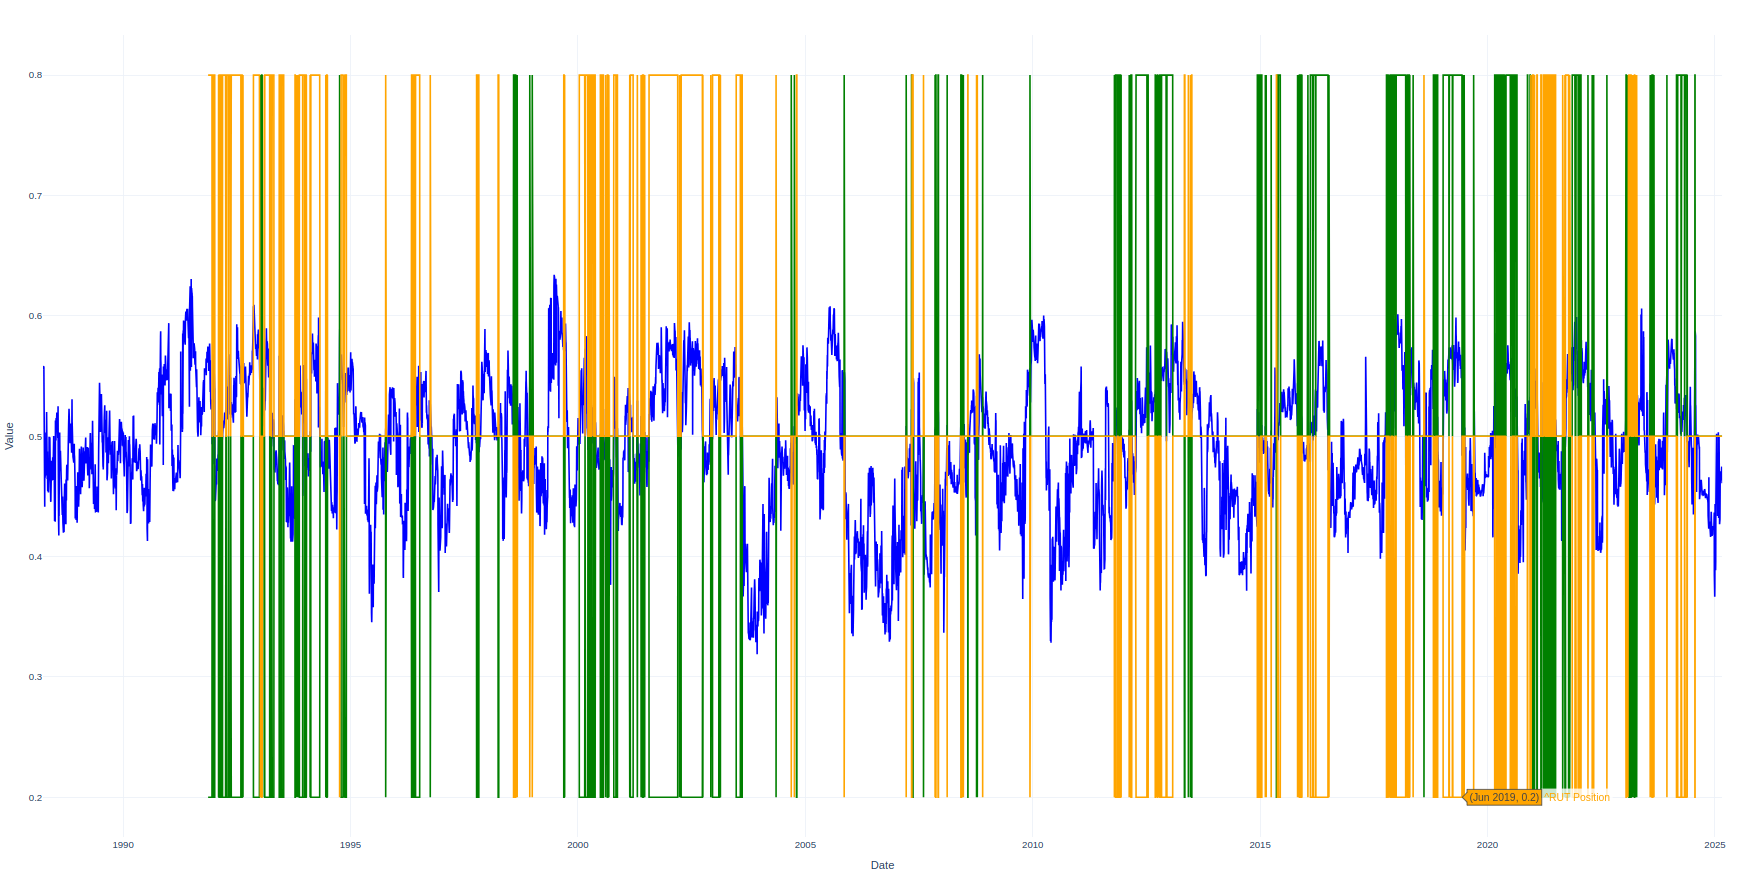
\includegraphics[width=0.8\textwidth]{img/position_switching.png}
    \caption{Composition of our portfolio
        (Russell 2000 in yellow, S\&P 500 in green) based on the inefficiency index, the blue line corresponds to the
        modified rolling hurst with a rolling window of 120 days. The position start to change in 1991-10-18 because we need
        4 years of data to compute the $\Delta\alpha_{\text{diff}}$. The portfolio is long only and the weights are adjusted daily.
        To comeback where you left off, see Section~\ref{sec:backtest_results}.}
    \label{fig:position_switching}
\end{figure}
\FloatBarrier

\subsection{Backtest different rolling window size results}

\begin{table}[!h]
    \centering
    \pgfplotstabletypeset[
        columns={Strategy,Annualized Return,Annualized Volatility,Sharpe,Max Drawdown},
        columns/Strategy/.style={string type,column name=Strategy},
        columns/Annualized Return/.style={column name=Annualized Return},
        columns/Annualized Volatility/.style={column name=Annualized Volatility},
        columns/Sharpe/.style={column name=Sharpe},
        columns/Max Drawdown /.style={column name=Max Drawdown}
    ]{data/backtest_results_window_120.csv}
    \caption{1991-11-15 to 2025-02-28 | Window size 120 days. To comeback where you left off, see Section~\ref{sec:backtest_results}.}
    \label{tab:performance_table_window_120}
\end{table}
\FloatBarrier

\begin{table}[!h]
    \centering
    \pgfplotstabletypeset[
        columns={Strategy,Annualized Return,Annualized Volatility,Sharpe,Max Drawdown},
        columns/Strategy/.style={string type,column name=Strategy},
        columns/Annualized Return/.style={column name=Annualized Return},
        columns/Annualized Volatility/.style={column name=Annualized Volatility},
        columns/Sharpe/.style={column name=Sharpe},
        columns/Max Drawdown /.style={column name=Max Drawdown}
    ]{data/backtest_results_window_252.csv}
    \caption{1991-11-15 to 2025-02-28 | Window size 252 days}
    \label{tab:performance_table_window_252}
\end{table}
\FloatBarrier

\begin{table}[!h]
    \centering
    \pgfplotstabletypeset[
        columns={Strategy,Annualized Return,Annualized Volatility,Sharpe,Max Drawdown},
        columns/Strategy/.style={string type,column name=Strategy},
        columns/Annualized Return/.style={column name=Annualized Return},
        columns/Annualized Volatility/.style={column name=Annualized Volatility},
        columns/Sharpe/.style={column name=Sharpe},
        columns/Max Drawdown /.style={column name=Max Drawdown}
    ]{data/backtest_results_window_504.csv}
    \caption{1991-11-15 to 2025-02-28 | Window size 504 days}
    \label{tab:performance_table_window_504}
\end{table}
\FloatBarrier

\begin{table}[!h]
    \centering
    \pgfplotstabletypeset[
        columns={Strategy,Annualized Return,Annualized Volatility,Sharpe,Max Drawdown},
        columns/Strategy/.style={string type,column name=Strategy},
        columns/Annualized Return/.style={column name=Annualized Return},
        columns/Annualized Volatility/.style={column name=Annualized Volatility},
        columns/Sharpe/.style={column name=Sharpe},
        columns/Max Drawdown /.style={column name=Max Drawdown}
    ]{data/backtest_results_window_1260.csv}
    \caption{1992-08-22-2025-02-28 | Window size 1260 days}
    \label{tab:performance_table_window_1260}
\end{table}
\FloatBarrier

\begin{table}[!h]
    \centering
    \pgfplotstabletypeset[
        columns={Strategy,Annualized Return,Annualized Volatility,Sharpe,Max Drawdown},
        columns/Strategy/.style={string type,column name=Strategy},
        columns/Annualized Return/.style={column name=Annualized Return},
        columns/Annualized Volatility/.style={column name=Annualized Volatility},
        columns/Sharpe/.style={column name=Sharpe},
        columns/Max Drawdown /.style={column name=Max Drawdown}
    ]{data/backtest_results_window_2520.csv}
    \caption{1997-06-18-2025-02-28 | Window size 2520 days}
    \label{tab:performance_table_window_2520}
\end{table}
\FloatBarrier

\section{References}

Lo, A.W. (1991). \textit{\href{http://www.e-m-h.org/Lo\_\_91.pdf}{Long-Term Memory in Stock Market Prices}}. \\

Mignon, V. (2003). \textit{\href{https://www.persee.fr/doc/ecop_0249-4744_1998_num_132_1_5909}{Méthodes d'estimation de l'exposant de Hurst. Application aux rentabilités boursières}}, Économie \& Prévision.

Kantelhardt, J.W., Zschiegner, S.A., Koscielny-Bunde, E., Bunde, A., Havlin, S., \& Stanley, H.E. (2002). \textit{Multifractal Detrended Fluctuation Analysis of Nonstationary Time Series}. \textit{Physica A: Statistical Mechanics and its Applications}, 316(1--4), 87--114.

Lukasz Czarnecki, Dariusz Grech, Multifractal dynamics of stock markets, 2009, Acta Physica Polonica Series.


Andrews, D.W.K. (1991). \textit{\href{https://www.jstor.org/stable/2938229}{Heteroskedasticity and Autocorrelation Consistent Covariance Matrix Estimation}}. \textit{Econometrica}, 59(3), 817-858.

Mandelbrot, B.B. and Wallis, J.R. (1968). "Noah, Joseph, and Operational Hydrology", \textit{Water Resources Research}, vol. 4, pp. 909--918.

Mandelbrot, B.B. (1973). "Le problème de la réalité des cycles lents et le syndrome de Joseph", \textit{Economie Appliquée}, vol. 26, pp. 349--365.

Mandelbrot, B.B. and Wallis, J.R. (1969a). "Some Long-Run Properties of Geophysical Records", \textit{Water Resources Research}, vol. 5, pp. 321--340.

Mandelbrot, B.B. and Wallis, J.R. (1969b). "Robustness of the Rescaled Range R/S in the Measurement of Noncyclic Long-Run Statistical Dependence", \textit{Water Resources Research}, vol. 5, pp. 967--988.

Mandelbrot, B.B. and Taqqu, M.S. (1979). "Robust R/S Analysis of Long-Run Serial Correlation", \textit{Bulletin of the International Statistical Institute}, vol. 48, pp. 69--104.

\end{document}
